\documentclass{acm_proc_article-sp}
\bibliographystyle{unsrt}

\begin{document}

\title{Cellular Automata for Artificial Life Games}
\numberofauthors{1}
\author{
% 1st. author
\alignauthor
Ian Holmes\\
       \affaddr{Department of Bioengineering}\\
       \affaddr{University of California}\\
       \affaddr{California, Berkeley}\\
       \email{ihh@berkeley.edu}
}
\date{30 November, 2013}

\maketitle
\begin{abstract}
Experimental turn-based multiplayer on mobile devices,
using cellular automata to implement models
from condensed-matter physics, mathematical biology,
and artificial life research
\end{abstract}

% A category with the (minimum) three required fields
%\category{H.4}{Information Systems Applications}{Miscellaneous}
%A category including the fourth, optional field follows...
%\category{D.2.8}{Software Engineering}{Metrics}[complexity measures, performance measures]


\section{Introduction}

Goal: 
build platform for experimental gameplay
using cellular automata to implement models
from condensed-matter physics, mathematical biology,
and Artificial Life ({\em A-Life})

\subsection{Cellular Automata}

\cite{Schiff2007}

\subsection{Artificial Life Models}

\cite{VonNeumannBook}

\cite{Conway}

\cite{Wireworld}

\cite{Langton}

\section{Simulation}

\subsection{Virtual Machine}

Low-level (machine code):
state machines.
Bitfields: fixed amount of dynamic storage, 16 bits given over to a type field that selects from a global program.
Remaining dynamic storage 48 bits, plus effectively unlimited read-only global storage.
Minimal generalization of lookup table, to facilitate partial matching of neighborhoods:
bitfield access, load-add-store, load-switch.

Low-level (assembly language):
Scheme. Generates (assembles) instructions for state machine.
Large built-in library for replicating patterns over Moore or von Neumann neighborhoods,
implementing reaction-diffusion models, implementing turtle-type agents, etc.

Higher-level (complex agent scripting):
Scheme. S-expression dynamic storage.

Board:
Square slab, $S \times S \times D$.
Isometric rendering.


\subsection{Polymers}

\cite{DoiEdwards}

As shown in Figure~\ref{fig:polymer}.

\begin{figure}
\fbox{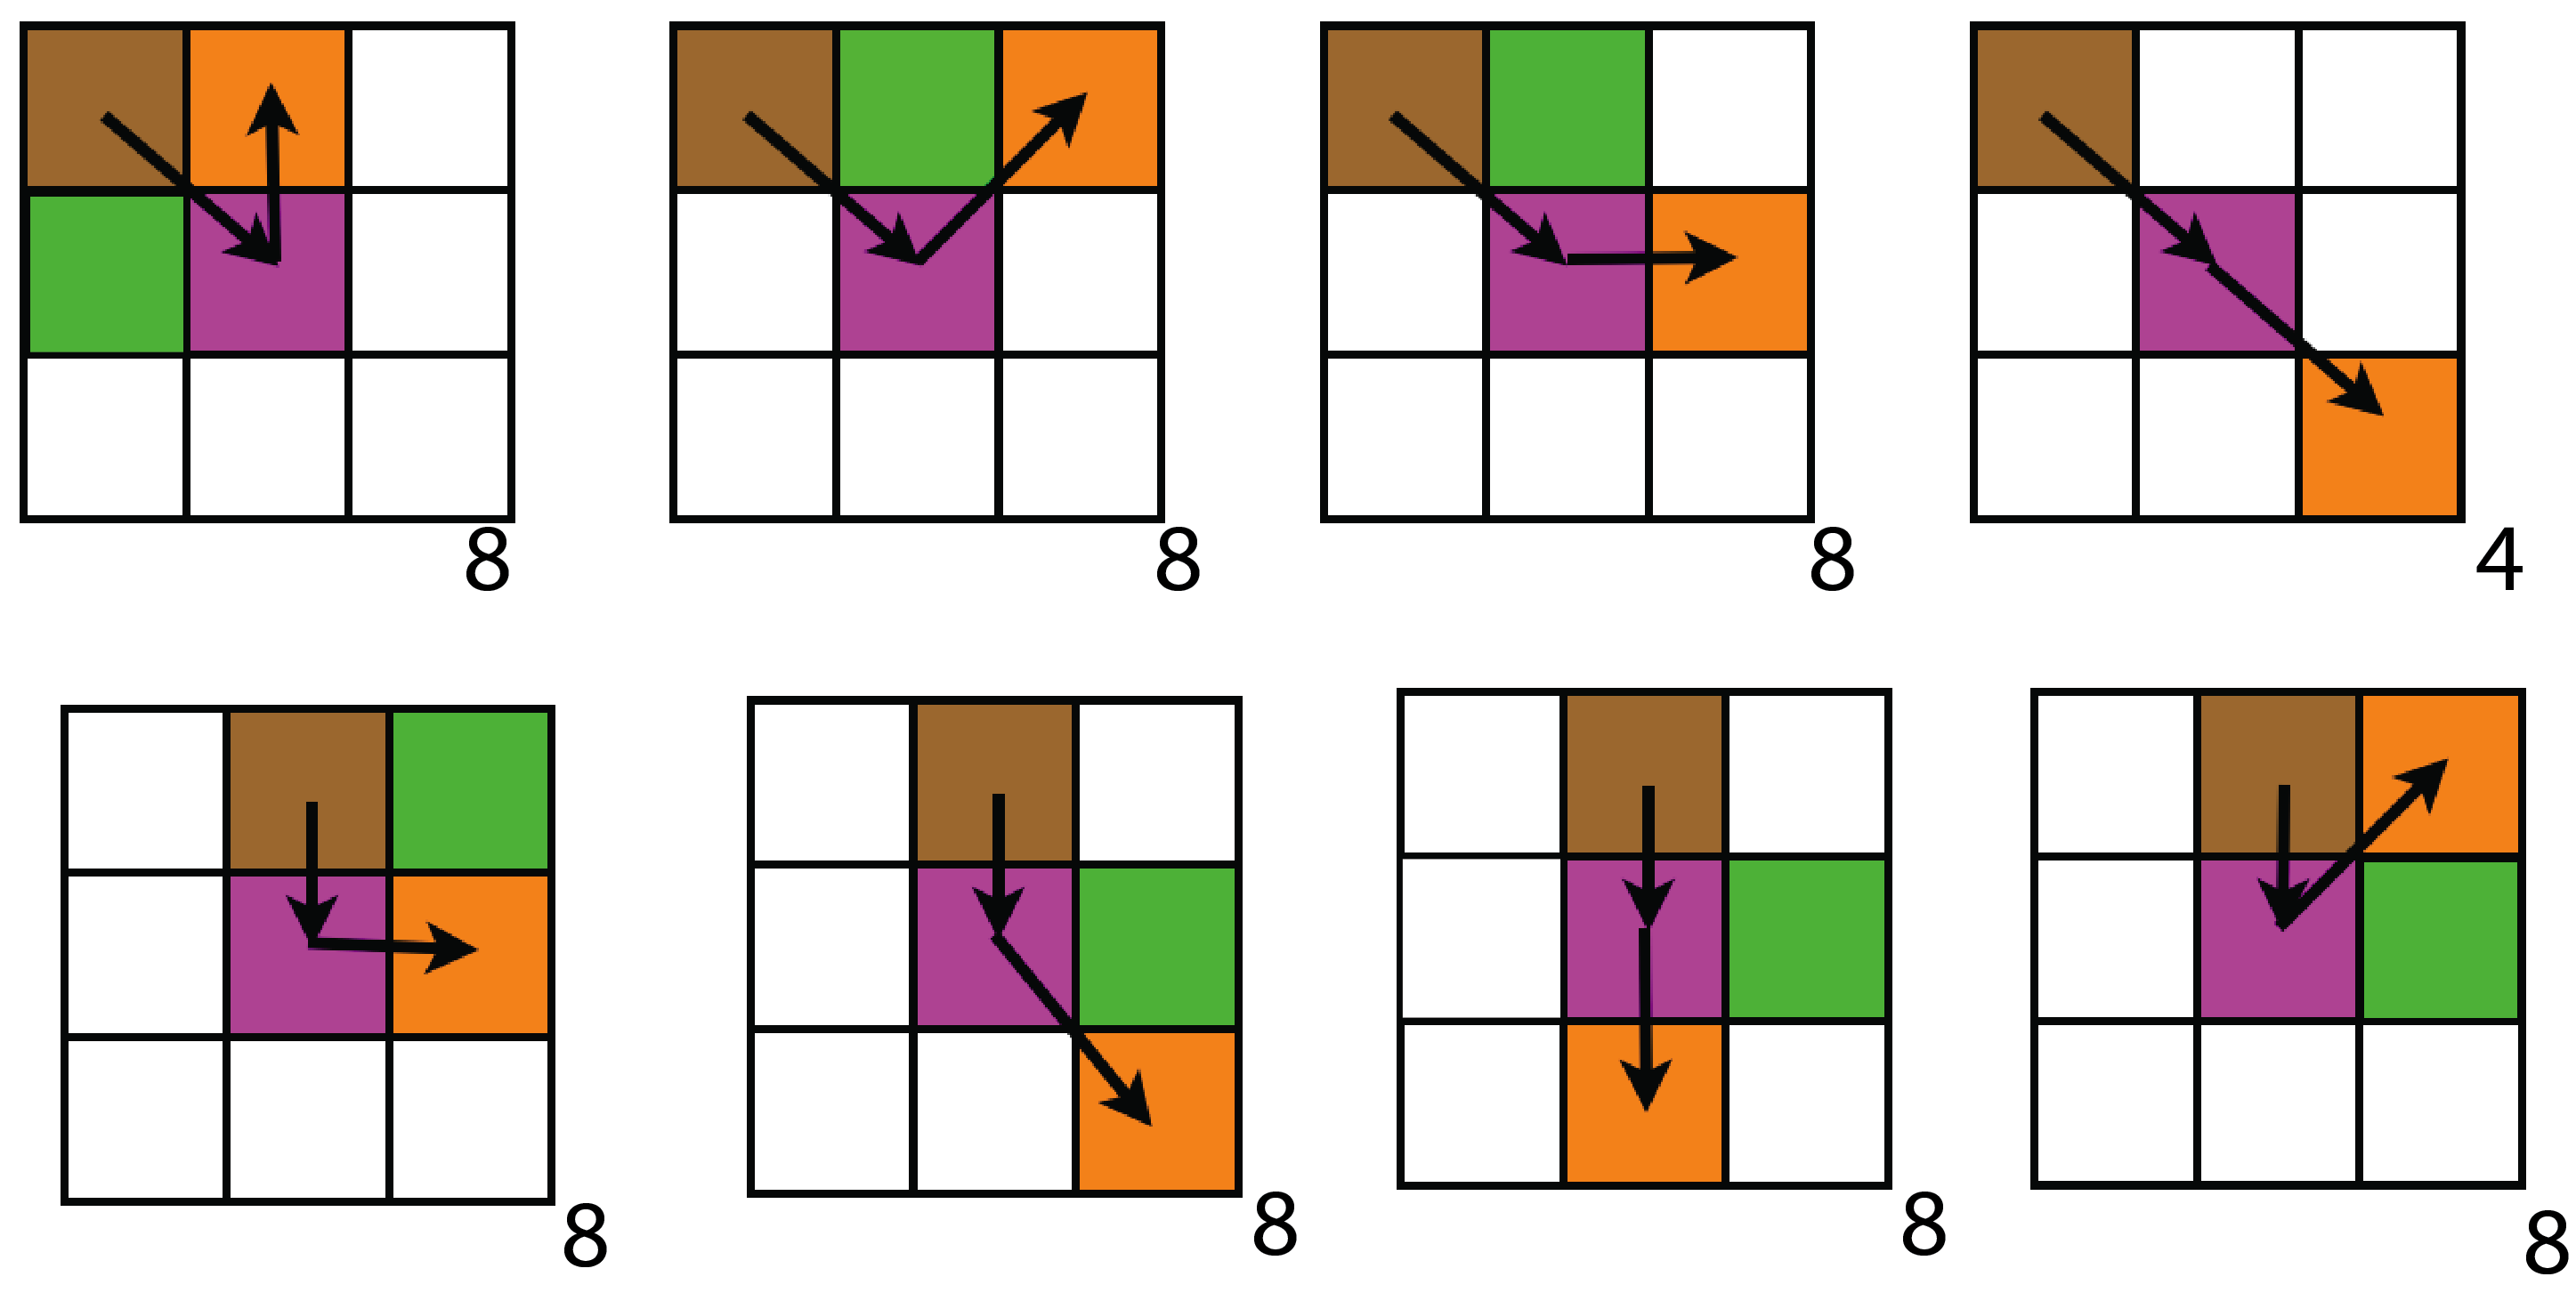
\includegraphics[width=\columnwidth]{Polymer.png}}
\caption{
\label{fig:polymer}
A few cases in the explicit automata-theoretic enumeration of polymer diffusion.
}
\end{figure}


\subsection{RNA Folding}

\cite{LeoniVanderzande2003,JostEveraers2010,ZaraPretti2007,GillespieMayneJiang2009}


As shown in Figure~\ref{fig:rna}.

\begin{figure}
\fbox{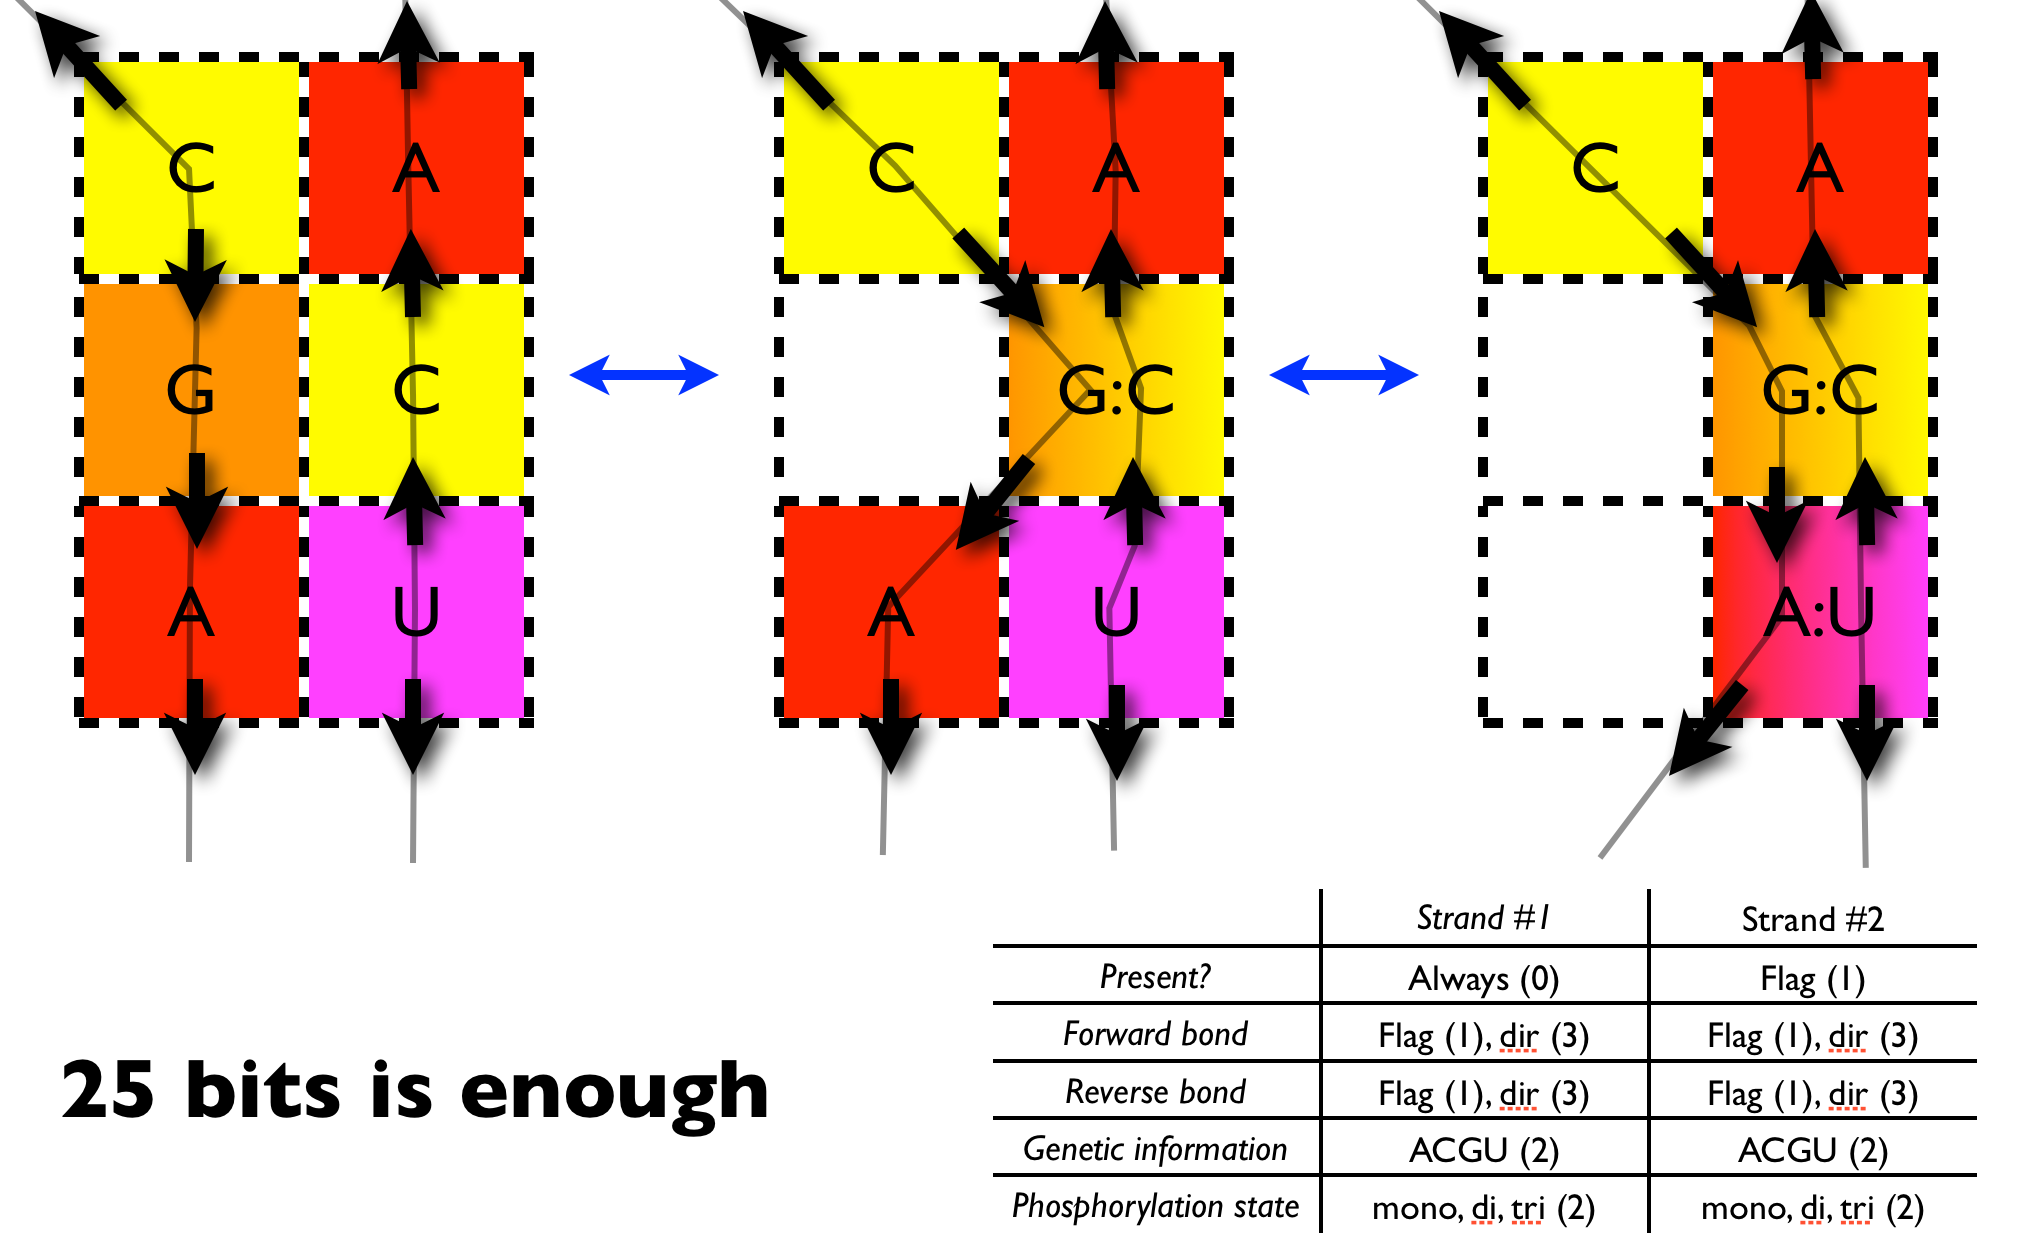
\includegraphics[width=\columnwidth]{RNA.png}}
\caption{
\label{fig:rna}
A sample case in the explicit automata-theoretic enumeration of RNA folding.
}
\end{figure}

\cite{Durbin98}

\subsection{Agent Patterns}

Tumble-swim: {\em E.coli}.
\cite{EcoliTumbleRoll}

Sudoku ant: push obstacle a random number of blocks before changing direction.
\cite{AntBehaviorNature}

Reaction-diffusion.
Directed diffusion.
Diffusion-limited aggregation.
\cite{DLA}

Lotka-Volterra (predator-prey) \cite{LotkaVolterra,SpatialLotkaVolterra}. RPS.
Ecosystem stability \cite{Quince}.

Population dynamics. \cite{WrightFisher}

\section{Game Design}

\subsection{Basic Play}

Like PAINT with live pixels.

Game goal: maintain dynamic equilibrium between three RPS species within a vesicle.

Multiplayer operation: RESTful server \cite{RESTthesis}, post lock, check board out/in.

Time-limited turns, minimum time between turns, max tool recharge per day.

Multiplayer goal: keep your population alive under attack.

Earn money from your population.

\subsection{Creating New Tools}

Spend money creating and using new reaction-diffusion particles and spray-tools.

\section{Implementation}

Gnu C, libXML, GDataXML, ChibiScheme, XCode, Catalyst (Perl).

\subsection{Acknowledgements}

Many thanks are due Alex Shinn, Richard Evans, Michael Mateas, Sean Eddy, Gerald Joyce, Chris Quince,
and Rudy Rucker for help and inspiration.


\bibliography{pzpaper}

\balancecolumns
% That's all folks!
\end{document}
